\subsubsection{Komponenter}
\paragraph{Motstand} \mbox{} \\
En motstand, også kalt resistor, er en komponent som begrenser strømmen.
Tenk på det som en kran du skrur igjen for å begrense antall elektroner som flyter forbi.
Det refererer også til et stoffs begrensede ledningsevne.
\\
Motstand noteres som $R$ (for resistance) og måles i ohm \SI{}{\ohm}.

\paragraph{Kondensator} \mbox{} \\
En kondensator (engelsk: capacitor) er en bøtte. Atpåtil en bøtte med hull i.
\\
Du fyller den med så mye vann du vil, men gjennom det lille hullet i bøtta kan bare en viss mengde vann renne.
\\\\
Kondensatorer brukes til å motstå forandring i spenning.
Med andre ord, holde spenning stabil.
\\
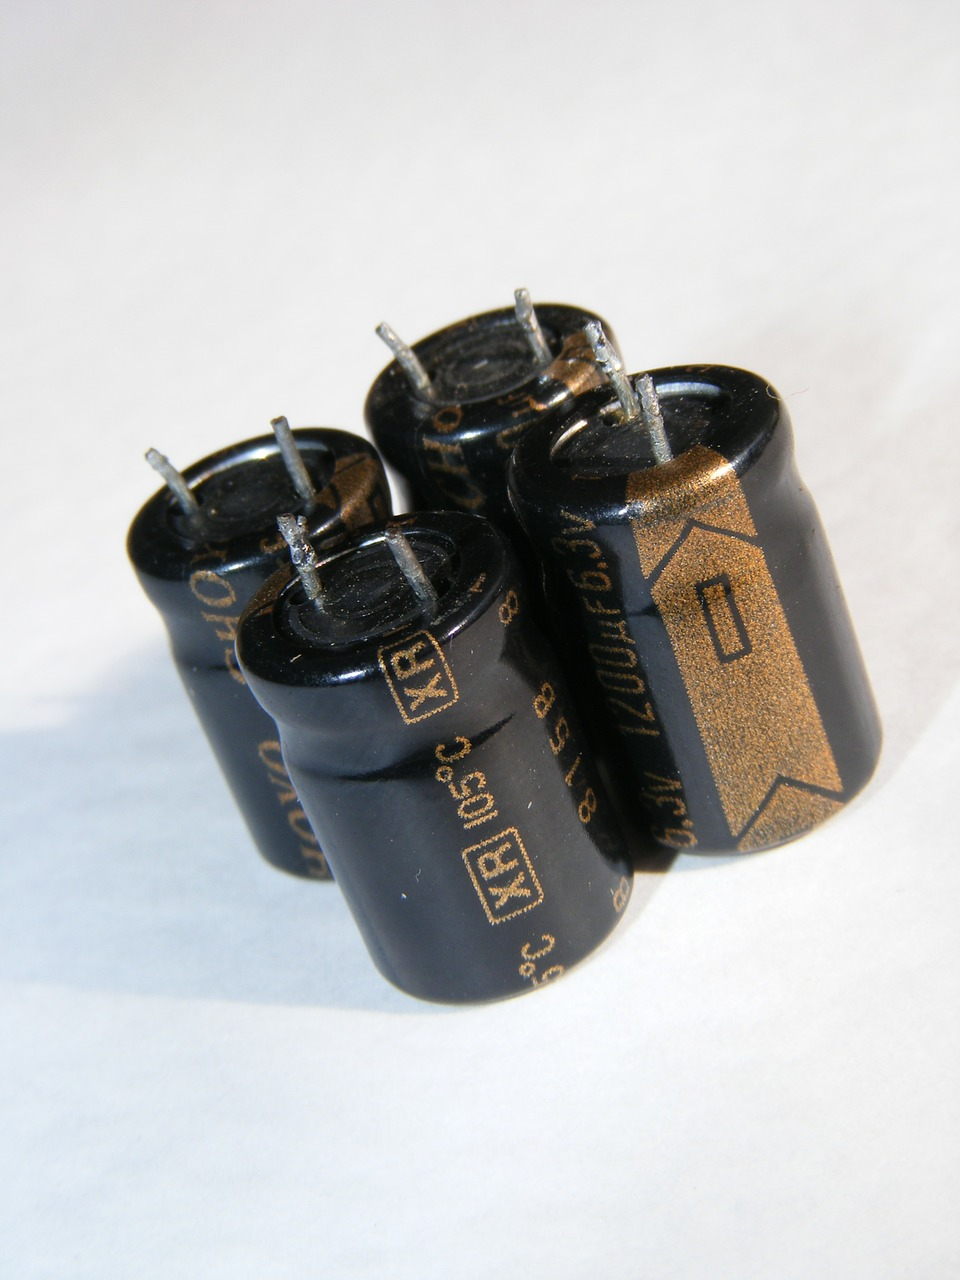
\includegraphics[width=0.25\textwidth]{./img/kondensator}

\paragraph{Spole} \mbox{} \\
En spole (engelsk: inductor) motstår forandring i strøm.
Det er likheter mellom funksjonen til en spole og en kondensator, men måten de fungerer på er forksjellig.
